\chapter{Thực nghiệm và đánh giá}
\label{ch:experiment}

Chương này trình bày thiết lập thực nghiệm và lần lượt trả lời ba câu hỏi nghiên cứu đã đặt ra, đánh giá hệ thống phát hiện ESG-washing đề xuất ở Chương~\ref{ch:method}.

%% ============================================================
%% 4.1 CÂU HỎI NGHIÊN CỨU
%% ============================================================



%% ============================================================
%% 4.2 DỮ LIỆU VÀ THIẾT LẬP THỰC NGHIỆM
%% ============================================================
\section{Thiết lập thực nghiệm}
\label{sec:exp_setup}

Toàn bộ quá trình huấn luyện và thực hiện pipeline được thực hiện trên nền tảng Google Colab với GPU T4 (15\,GB VRAM), RAM 12\,GB.

\subsection{Tập dữ liệu}
\label{subsec:dataset}

Tập dữ liệu được xây dựng từ báo cáo thường niên của 10 ngân hàng thương mại Việt Nam trong giai đoạn 2020--2024, tổng cộng 50 quan sát ngân hàng-năm (chi tiết quy trình thu thập và tiền xử lý xem Mục~\ref{sec:data_preparation}). Sau khi phân đoạn và lọc, corpus gồm 113.986 câu, trong đó 32.313 câu được phân loại thuộc nhóm ESG.

Dữ liệu huấn luyện cho hai bộ phân loại được chia theo tỉ lệ 80/10/10 với phân tầng theo nhãn. Bảng~\ref{tab:data_split} tóm tắt quy mô các tập.

\begin{table}[H]
\centering
\caption{Quy mô tập dữ liệu huấn luyện, xác thực và kiểm thử.}
\label{tab:data_split}
\begin{tabular}{lrrr}
\toprule
\textbf{Bộ phân loại} & \textbf{Train} & \textbf{Val} & \textbf{Test} \\
\midrule
Chủ đề ESG (6 nhãn)        & 91.188 & 11.399 & 11.399 \\
Mức độ hành động (3 nhãn)   & 25.808 &  3.226 &  3.226 \\
\bottomrule
\end{tabular}
\end{table}

Phân phối nhãn của tập huấn luyện được trình bày trong Bảng~\ref{tab:label_dist}. Để xử lý mất cân bằng, nghiên cứu sử dụng trọng số lớp theo phương pháp \textit{sqrt-inverse}.

\begin{table}[H]
\centering
\caption{Phân phối nhãn trong tập huấn luyện.}
\label{tab:label_dist}
\begin{tabular}{lrr|lrr}
\toprule
\multicolumn{3}{c|}{\textbf{Chủ đề ESG}} & \multicolumn{3}{c}{\textbf{Mức độ hành động}} \\
\textbf{Nhãn} & \textbf{Số mẫu} & \textbf{\%} & \textbf{Nhãn} & \textbf{Số mẫu} & \textbf{\%} \\
\midrule
Non\_ESG      & 65.338 & 71,6 & Indeterminate & 16.756 & 64,9 \\
G             & 13.450 & 14,7 & Implemented   &  8.322 & 32,3 \\
S\_labor      &  4.470 &  4,9 & Planning      &    730 &  2,8 \\
S\_product    &  3.904 &  4,3 &               &        &      \\
E             &  2.429 &  2,7 &               &        &      \\
S\_community  &  1.597 &  1,8 &               &        &      \\
\bottomrule
\end{tabular}
\end{table}


\subsection{Cấu hình siêu tham số}
\label{subsec:hyperparams}

Mô hình nền tảng là PhoBERT-base với 135 triệu tham số. Các siêu tham số được xác định qua quá trình tinh chỉnh bằng Optuna với thuật toán TPE (Tree-structured Parzen Estimator). Không gian tìm kiếm gồm sáu chiều được liệt kê trong Bảng~\ref{tab:tuning_space}. Kết quả của quá trình tối ưu siêu tham số được tổng hợp trong Bảng~\ref{tab:hyperparams}.

\begin{table}[H]
\centering
\caption{Không gian tìm kiếm siêu tham số trong Optuna.}
\label{tab:tuning_space}
\begin{tabular}{llr}
\toprule
\textbf{Siêu tham số} & \textbf{Kiểu phân phối} & \textbf{Phạm vi} \\
\midrule
\texttt{learning\_rate}      & Log-uniform & $[10^{-5},\ 5 \times 10^{-5}]$ \\
\texttt{batch\_size}         & Categorical & $\{8,\ 16,\ 32\}$ \\
\texttt{max\_length}         & Categorical & $\{128,\ 256\}$ \\
\texttt{weight\_decay}       & Uniform     & $[0{,}00,\ 0{,}10]$ \\
\texttt{num\_epochs}         & Integer     & $[3,\ 10]$ \\
\texttt{constraint\_lambda}  & Uniform     & $[0{,}05,\ 0{,}70]$ \\
\bottomrule
\end{tabular}
\end{table}

\begin{table}[H]
\centering
\caption{Cấu hình siêu tham số huấn luyện.}
\label{tab:hyperparams}
\begin{tabular}{lrr}
\toprule
\textbf{Tham số} & \textbf{Chủ đề ESG} & \textbf{Hành động} \\
\midrule
Mô hình nền tảng        & \multicolumn{2}{c}{PhoBERT-base (135M params)} \\
Max length (token)   & 128  & 128  \\
epoch                & 5    & 5    \\
Batch size (train/eval) & 16 / 32 & 16 / 32 \\
Learning rate           & $1{,}951 \times 10^{-5}$ & $2{,}004 \times 10^{-5}$ \\
Weight decay            & 0,0289 & 0,0456 \\
Warmup ratio            & 10\%  & 10\%  \\
Early stopping patience & \multicolumn{2}{c}{2 epoch} \\
Seed                    & \multicolumn{2}{c}{42} \\
\midrule
\multicolumn{3}{l}{\textit{Neuro-symbolic}} \\
$\lambda$ (constraint loss) & 0,2798 & 0,1798 \\
\bottomrule
\end{tabular}
\end{table}

\section{Trả lời câu hỏi một: Hiệu quả phương pháp neuro-symbolic}
\label{sec:rq1}

Phần này đánh giá hiệu quả của phương pháp neuro-symbolic so với cấu hình Baseline (PhoBERT fine-tuning thuần, không có ràng buộc ký hiệu).


\subsubsection{Phân loại chủ đề ESG}
\label{subsec:topic_baseline_vs_neuro}

\begin{table}[H]
\centering
\caption{Kết quả phân loại chủ đề ESG trên tập kiểm thử.}
\label{tab:topic_perclass}
\small
\begin{tabular}{l|rrr|rrr}
\toprule
 & \multicolumn{3}{c|}{\textbf{Baseline}} & \multicolumn{3}{c}{\textbf{Neuro-Symbolic}} \\
\textbf{Nhãn} & \textbf{P} & \textbf{R} & \textbf{F1} & \textbf{P} & \textbf{R} & \textbf{F1} \\
\midrule
E            & 0,70 & 0,77 & 0,73 & 0,74 & 0,84 & \textbf{0,79} \\
S\_labor     & 0,76 & 0,81 & 0,78 & 0,82 & 0,89 & \textbf{0,85} \\
S\_community & 0,70 & 0,77 & 0,73 & 0,78 & 0,83 & \textbf{0,80} \\
S\_product   & 0,60 & 0,72 & 0,66 & 0,68 & 0,80 & \textbf{0,73} \\
G            & 0,75 & 0,83 & 0,79 & 0,81 & 0,92 & \textbf{0,86} \\
Non\_ESG     & 0,91 & 0,87 & 0,89 & 0,97 & 0,92 & \textbf{0,95} \\
\midrule
\textbf{Macro avg} & 0,74 & 0,79 & 0,76 & 0,80 & 0,87 & \textbf{0,83} \\
\textbf{Accuracy}  & \multicolumn{3}{c|}{0,870} & \multicolumn{3}{c}{\textbf{0,911}} \\
\bottomrule
\end{tabular}
\end{table}

\begin{figure}[H]
    \centering
    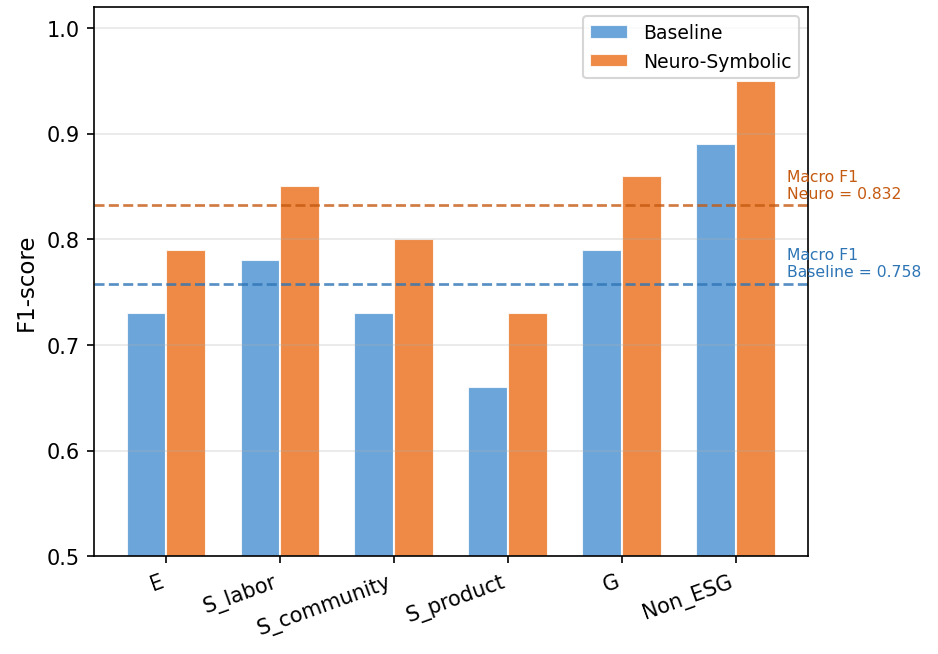
\includegraphics[width=0.75\textwidth]{figures/rq1_perclass_topic.png}
    \caption{So sánh F1-score bộ phân loại chủ đề ESG theo từng nhãn giữa Baseline và Neuro-Symbolic.}
    \label{fig:rq1_perclass}
\end{figure}

Cấu hình Neuro-Symbolic vượt trội Baseline trên toàn bộ sáu nhãn với mức cải thiện Macro F1 là 0,832 so với 0,758 trên tập kiểm thử. Mức cải thiện lớn nhất ở nhãn G (0,79 $\to$ 0,86) và S\_labor (0,78 $\to$ 0,85), phản ánh lợi ích của các ràng buộc loại trừ lẫn nhau giữa nhóm nhãn E/S/G. Nhãn Non\_ESG cũng được cải thiện rõ (0,89 $\to$ 0,95), cho thấy ràng buộc exclusion hiệu quả trong việc giảm false positive.

\subsubsection{Phân loại mức độ hành động}
\label{subsec:action_baseline_vs_neuro}

\begin{table}[H]
\centering
\caption{Kết quả phân loại mức độ hành động trên tập kiểm thử.}
\label{tab:action_perclass}
\begin{tabular}{l|rrr|rrr}
\toprule
 & \multicolumn{3}{c|}{\textbf{Baseline}} & \multicolumn{3}{c}{\textbf{Neuro-Symbolic}} \\
\textbf{Nhãn} & \textbf{P} & \textbf{R} & \textbf{F1} & \textbf{P} & \textbf{R} & \textbf{F1} \\
\midrule
Implemented   & 0,81 & 0,80 & 0,80 & 0,86 & 0,84 & \textbf{0,85} \\
Planning      & 0,57 & 0,71 & 0,63 & 0,65 & 0,76 & \textbf{0,70} \\
Indeterminate & 0,88 & 0,88 & 0,88 & 0,91 & 0,92 & \textbf{0,92} \\
\midrule
\textbf{Macro avg} & 0,75 & 0,80 & 0,77 & 0,81 & 0,84 & \textbf{0,82} \\
\textbf{Accuracy}  & \multicolumn{3}{c|}{0,862} & \multicolumn{3}{c}{\textbf{0,887}} \\
\bottomrule
\end{tabular}
\end{table}

\begin{figure}[H]
    \centering
    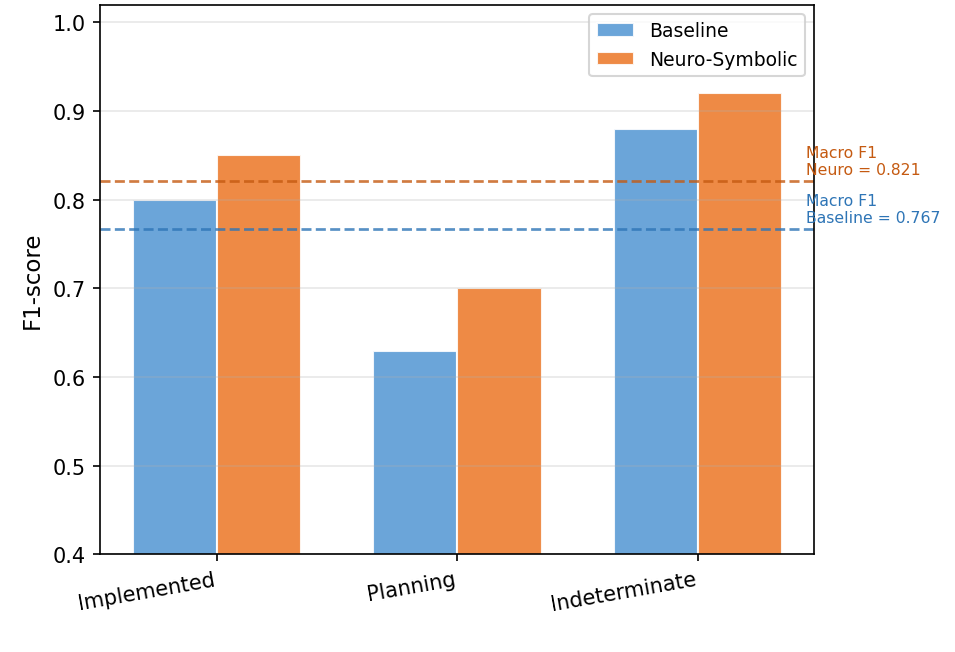
\includegraphics[width=0.75\textwidth]{figures/rq1_perclass_action.png}
    \caption{So sánh F1-score bộ phân loại chủ đề ESG theo từng nhãn giữa Baseline và Neuro-Symbolic.}
    \label{fig:rq1_perclass}
\end{figure}

Cấu hình Neuro-Symbolic đạt Macro F1 là 0,821 cao hơn so với Baseline là 0,767 trên tập kiểm thử. Đáng chú ý nhất là cải thiện trên nhãn thiểu số Planning: F1 tăng từ 0,63 lên 0,70, nhờ ràng buộc ký hiệu cung cấp tín hiệu trực tiếp để phân biệt Planning và Indeterminate. Recall trên Planning tăng từ 0,71 lên 0,76, cho thấy mô hình bỏ sót ít câu kế hoạch hơn.

Phương pháp neuro-symbolic kết hợp PhoBERT và quy tắc ký hiệu ESG đã cho thấy kết quả tốt hơn so với phương pháp Baseline trên cả hai bài toán phân loại. Với bộ phân loại chủ đề ESG, Neuro-Symbolic đạt Macro F1 = 0,832, với cải thiện đồng đều trên tất cả 6 nhãn. Với bộ phân loại hành động, Neuro-Symbolic đạt Macro F1 = 0,821, đặc biệt nổi bật trên nhãn thiểu số Planning (F1: 0,63 $\to$ 0,70). Hàm mất mát ngữ nghĩa đóng vai trò chuẩn hoá hiệu quả, đặc biệt có lợi khi dữ liệu mất cân bằng và ranh giới nhãn phụ thuộc tri thức chuyên biệt.


%% ============================================================
%% 4.3 TRẢ LỜI RQ2
%% ============================================================
\section{Trả lời câu hỏi hai: Liên kết bằng chứng ngữ nghĩa}
\label{sec:rq2}

Nghiên cứu so sánh ba phương pháp liên kết bằng chứng trên toàn bộ 32.313 câu ESG:

\begin{enumerate}
    \item \textbf{NLI}: Truy xuất ứng viên bằng TF-IDF + cosine similarity, sau đó xác minh bằng mô hình NLI (mDeBERTa-v3-base-xnli). Bằng chứng chỉ được chấp nhận khi NLI phán định \textit{entailment}.
    \item \textbf{Window context}: Truy xuất bằng chứng trong cửa sổ ngữ cảnh cố định (5 câu trước và sau), không sử dụng NLI.
    \item \textbf{No-NLI}: Truy xuất ứng viên bằng TF-IDF + cosine similarity, chấp nhận tất cả ứng viên vượt ngưỡng similarity.
\end{enumerate}

Tỉ lệ câu có bằng chứng là 24,6\% cho cả ba phương pháp, điều này phản ánh thực tế rằng phần lớn tuyên bố ESG trong báo cáo thường niên thiếu bằng chứng cụ thể đi kèm.

Phương pháp NLI đạt similarity trung bình 0,7249, thấp hơn nhẹ so với No-NLI (0,7316) vì bước xác minh NLI loại bỏ một số cặp có similarity cao nhưng không được có tính suy luận. Chỉ 32,8\% cặp tuyên bố-bằng chứng được NLI xác định là \textit{entailment}, trong khi 2,93\% được xác định \textit{contradiction}. Điều này cho thấy phần lớn các cặp thuộc nhóm \textit{neutral} --- bằng chứng có liên quan về chủ đề nhưng không trực tiếp xác nhận tuyên bố.

Bước xác minh NLI đóng vai trò quan trọng trong việc nâng cao chất lượng liên kết bằng chứng. Khi không có NLI, hệ thống chỉ dựa trên cosine similarity --- một độ đo tương đồng bề mặt không phân biệt được giữa \textit{entailment} (hỗ trợ) và \textit{contradiction} (mâu thuẫn). Ví dụ, câu tuyên bố \textit{``Ngân hàng cam kết giảm 30\% phát thải carbon''} và câu bằng chứng \textit{``Phát thải carbon của ngân hàng tăng 15\% trong năm 2023''} có cosine similarity cao (cùng chủ đề phát thải carbon) nhưng quan hệ NLI là \textit{contradiction}.

Tỉ lệ contradiction 2,93\% cho thấy cơ chế NLI phát hiện và loại bỏ một lượng nhỏ nhưng quan trọng các trường hợp bằng chứng ngược --- những trường hợp mà nếu bỏ qua sẽ làm giảm nghiêm trọng chất lượng đánh giá nguy cơ ESG-washing.

Phương pháp liên kết bằng chứng ngữ nghĩa hai giai đoạn (semantic retrieval + NLI verification) cải thiện chất lượng liên kết so với phương pháp cửa sổ ngữ cảnh. Cụ thể: (1) Truy xuất ngữ nghĩa đạt similarity cao hơn cửa sổ (+11,8\%, 0,7249 so với 0,6483); (2) NLI xác minh giúp loại bỏ 2,93\% cặp mâu thuẫn và phân biệt được giữa bằng chứng hỗ trợ (entailment, 32,8\%) và bằng chứng trung lập; (3) Kết quả cho thấy phần lớn tuyên bố ESG trong báo cáo thường niên ngân hàng Việt Nam (75,4\%) thiếu bằng chứng cụ thể.

\subsection{Phân bố loại bằng chứng}
\label{subsec:evidence_type_dist}

Bên cạnh việc đánh giá sự hiện diện của bằng chứng, hệ thống còn gán nhãn loại bằng chứng cho toàn bộ 119.733 câu trong ngữ liệu. Bảng~\ref{tab:evidence_type_dist} trình bày phân bố bốn loại bằng chứng được phát hiện.

\begin{table}[H]
\centering
\caption{Phân bố loại bằng chứng trên toàn ngữ liệu (119.733 câu). Một câu có thể thuộc nhiều loại cùng lúc.}
\label{tab:evidence_type_dist}
\small
\begin{tabular}{lrr}
\toprule
\textbf{Loại bằng chứng} & \textbf{Số câu} & \textbf{Tỉ lệ (\%)} \\
\midrule
KPI         & 52.881 & 44,2\% \\
Time\_bound & 41.523 & 34,7\% \\
Standard    & 21.552 & 18,0\% \\
Third\_party &  9.579 &  8,0\% \\
\midrule
Ít nhất một loại & 68.149 & 56,9\% \\
\bottomrule
\end{tabular}
\end{table}

KPI là loại phổ biến nhất (44,2\%), phản ánh thực tế rằng báo cáo thường niên ngân hàng chứa lượng lớn dữ liệu định lượng --- con số tài chính, tỉ lệ phần trăm, và chỉ số đo lường hoạt động. Time\_bound đứng thứ hai (34,7\%), cho thấy xu hướng đề cập thời gian cụ thể (năm, quý, giai đoạn) phổ biến trong văn phong báo cáo. Standard (18,0\%) tập trung chủ yếu tại các phần ESG chuyên biệt, nơi ngân hàng trình bày sự tuân thủ GRI, TCFD, hay các quy định NHNN. Third\_party là loại hiếm nhất (8,0\%), phù hợp với thực tế rằng xác minh độc lập --- kiểm toán bởi Big4, chứng nhận Bureau Veritas --- chỉ xuất hiện trong một số ít phần báo cáo.

Trong số 32.313 câu ESG, 24,6\% (7.949 câu) có bằng chứng liên kết (support $= 1$). So sánh với phân bố toàn ngữ liệu, các câu được liên kết bằng chứng thể hiện tập trung cao hơn vào KPI và Third\_party --- những loại bằng chứng mang tính kiểm chứng cao và thường đi kèm với tuyên bố Implemented. Điều này nhất quán với kết quả phân tích tương quan: tỉ lệ bằng chứng tương quan âm mạnh với EWRI ($r = -0{,}77$), tức là các tuyên bố có bằng chứng KPI hoặc Third\_party cụ thể giúp giảm rủi ro washing rõ rệt hơn so với bằng chứng Time\_bound hay Standard đơn thuần.

\section{Trả lời câu hỏi ba: Phân tích chỉ số EWRI}
\label{sec:rq3}

\subsection{Tổng quan kết quả EWRI}
\label{subsec:ewri_overview}

Kết quả tổng hợp chỉ số EWRI được tính cho 50 quan sát ngân hàng cho thấy EWRI trung bình = 35,15 $\pm$ 3,94 (thang điểm 0--100), phạm vi từ 28,67 đến 53,01.

\begin{table}[H]
\centering
\caption{Phân rã đóng góp EWRI theo thành phần nhãn hành động.}
\label{tab:ewri_decomposition}
\begin{tabular}{lccc}
\toprule
\textbf{Thành phần} & \textbf{Đóng góp TB} & \textbf{\% EWRI} & \textbf{Std} \\
\midrule
Indeterminate & 34,55 & 98,3\% & 3,97 \\
Implemented   &  0,36 &  1,0\% & 0,08 \\
Planning      &  0,24 &  0,7\% & 0,15 \\
\bottomrule
\end{tabular}
\end{table}

Thành phần Indeterminate chiếm đến 98,3\% tổng điểm EWRI, phản ánh thực tế rằng phần lớn tuyên bố ESG trong báo cáo ngân hàng Việt Nam ở trạng thái mơ hồ --- không rõ đã thực hiện hay mới chỉ là dự định. Đây chính là nguồn rủi ro washing chính: các phát biểu thiếu tính cụ thể, không có cam kết thời gian rõ ràng và không kèm bằng chứng kiểm chứng.

\begin{figure}[H]
    \centering
    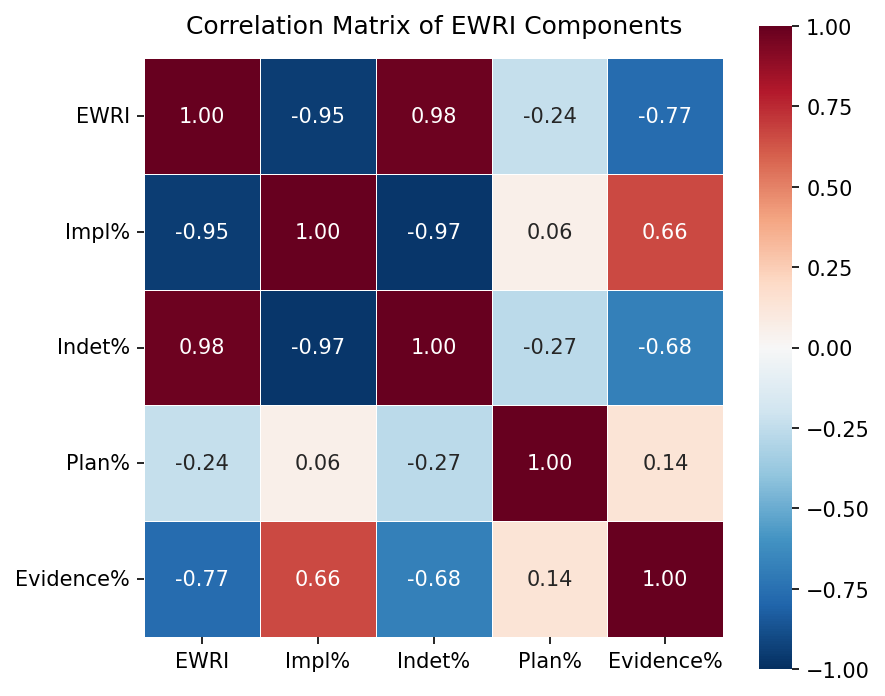
\includegraphics[width=0.6\textwidth]{figures/correlation_heatmap.png}
    \caption{Ma trận tương quan giữa EWRI và các thành phần.}
    \label{fig:correlation_heatmap}
\end{figure}

Các nhận định chính từ phân tích ma trận tương quan trên như sau:

\begin{itemize}
    \item EWRI tương quan dương rất mạnh với tỉ lệ Indeterminate ($r = 0{,}98$) và tương quan âm rất mạnh với tỉ lệ Implemented ($r = -0{,}95$). Điều này xác nhận rằng nhãn hành động --- đặc biệt là sự phân biệt giữa cam kết đã thực hiện và cam kết mơ hồ --- là yếu tố quyết định chính của EWRI.
    \item Tỉ lệ có bằng chứng hỗ trợ tương quan âm với EWRI ($r = -0{,}77$): ngân hàng có tỉ lệ câu được hỗ trợ bằng chứng cao hơn có xu hướng đạt EWRI thấp hơn.
    \item Tỉ lệ Planning không có tương quan đáng kể với EWRI ($r = -0{,}24$), tức là tỉ lệ câu Planning trong báo cáo không dự báo được mức EWRI của ngân hàng.
\end{itemize}

\subsection{Phân tích ESG-washing đối với các ngân hàng}
\label{subsec:bank_ranking}

Dưới đây là xếp hạng 10 ngân hàng theo EWRI trung bình giai đoạn 2020--2024:

\begin{figure}[H]
    \centering
    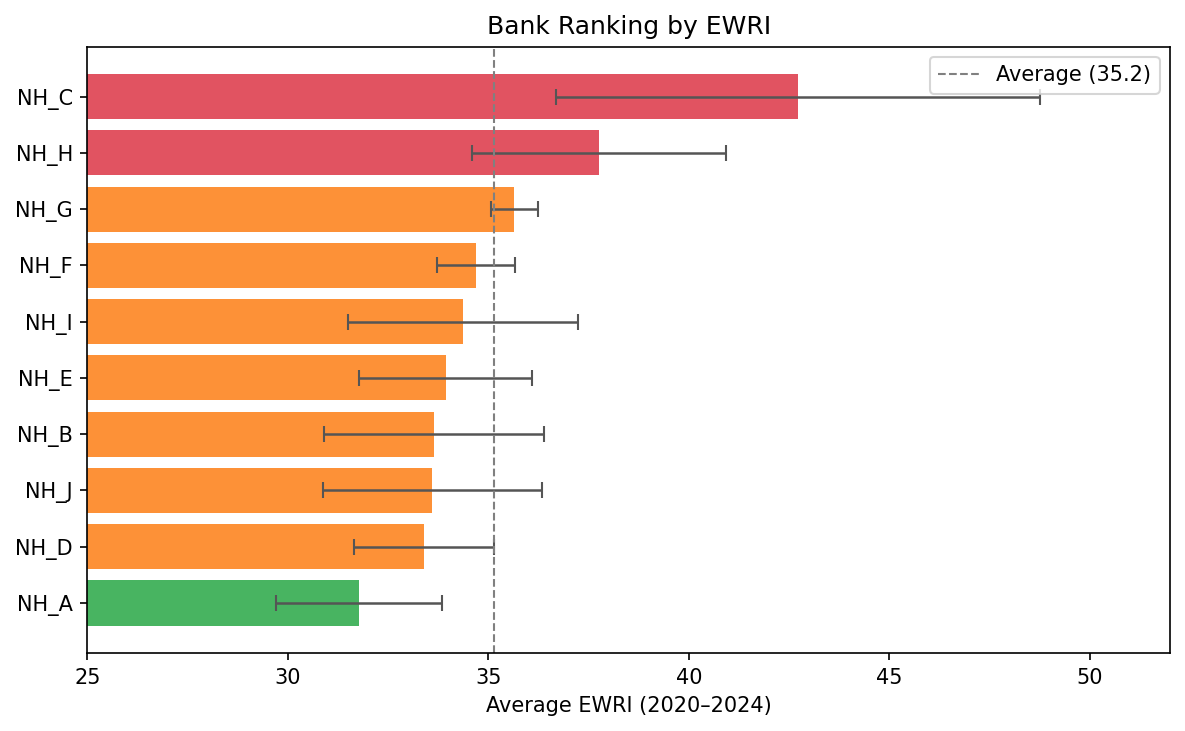
\includegraphics[width=0.75\textwidth]{figures/bank_ranking.png}
    \caption{Xếp hạng ngân hàng theo EWRI trung bình (2020--2024). Ngân hàng có EWRI thấp hơn được đánh giá minh bạch ESG tốt hơn.}
    \label{fig:bank_ranking}
\end{figure}

\begin{table}[H]
\centering
\caption{Chi tiết xếp hạng ngân hàng theo EWRI trung bình (2020--2024). $\bar{R}_I$: tỉ lệ Implemented; $\bar{R}_{In}$: tỉ lệ Indeterminate; $\bar{R}_E$: tỉ lệ có bằng chứng.}
\label{tab:bank_ranking_detail}
\small
\begin{tabular}{clcccccc}
\toprule
\textbf{Hạng} & \textbf{Ngân hàng} & \textbf{Số lượng câu} & \textbf{EWRI} & \textbf{Std} & \textbf{$\bar{R}_I$} & \textbf{$\bar{R}_{In}$} & \textbf{$\bar{R}_E$} \\
\midrule
1  & NH\_A  & 1.544 & 31,77 & 2,06 & 36,8\% & 60,5\% & 30,1\% \\
2  & NH\_D  & 3.485 & 33,40 & 1,74 & 33,7\% & 63,0\% & 30,3\% \\
3  & NH\_J  & 4.513 & 33,60 & 2,73 & 34,9\% & 62,3\% & 25,2\% \\
4  & NH\_B  & 4.330 & 33,65 & 2,75 & 34,3\% & 62,2\% & 25,6\% \\
5  & NH\_E  & 1.716 & 33,93 & 2,16 & 34,4\% & 64,2\% & 25,8\% \\
6  & NH\_I  & 5.155 & 34,37 & 2,87 & 33,7\% & 64,2\% & 24,4\% \\
7  & NH\_F  & 3.898 & 34,69 & 0,97 & 32,8\% & 64,8\% & 23,0\% \\
8  & NH\_G  & 4.303 & 35,65 & 0,59 & 29,3\% & 66,9\% & 24,6\% \\
9  & NH\_H  & 1.550 & 37,76 & 3,16 & 27,4\% & 70,4\% & 22,1\% \\
10 & NH\_C  & 1.766 & 42,72 & 6,03 & 21,9\% & 76,7\% & 18,4\% \\
\bottomrule
\end{tabular}
\end{table}

NH\_A dẫn đầu với EWRI thấp nhất (31,77), nhờ tỉ lệ Implemented cao nhất (36,8\%) và tỉ lệ Indeterminate thấp nhất (60,5\%). NH\_C xếp cuối với EWRI = 42,72 (chênh 10,95 điểm so với NH\_A), trong đó năm 2020 đạt EWRI = 53,01 --- mức cao nhất toàn tập.

\begin{figure}[H]
    \centering
    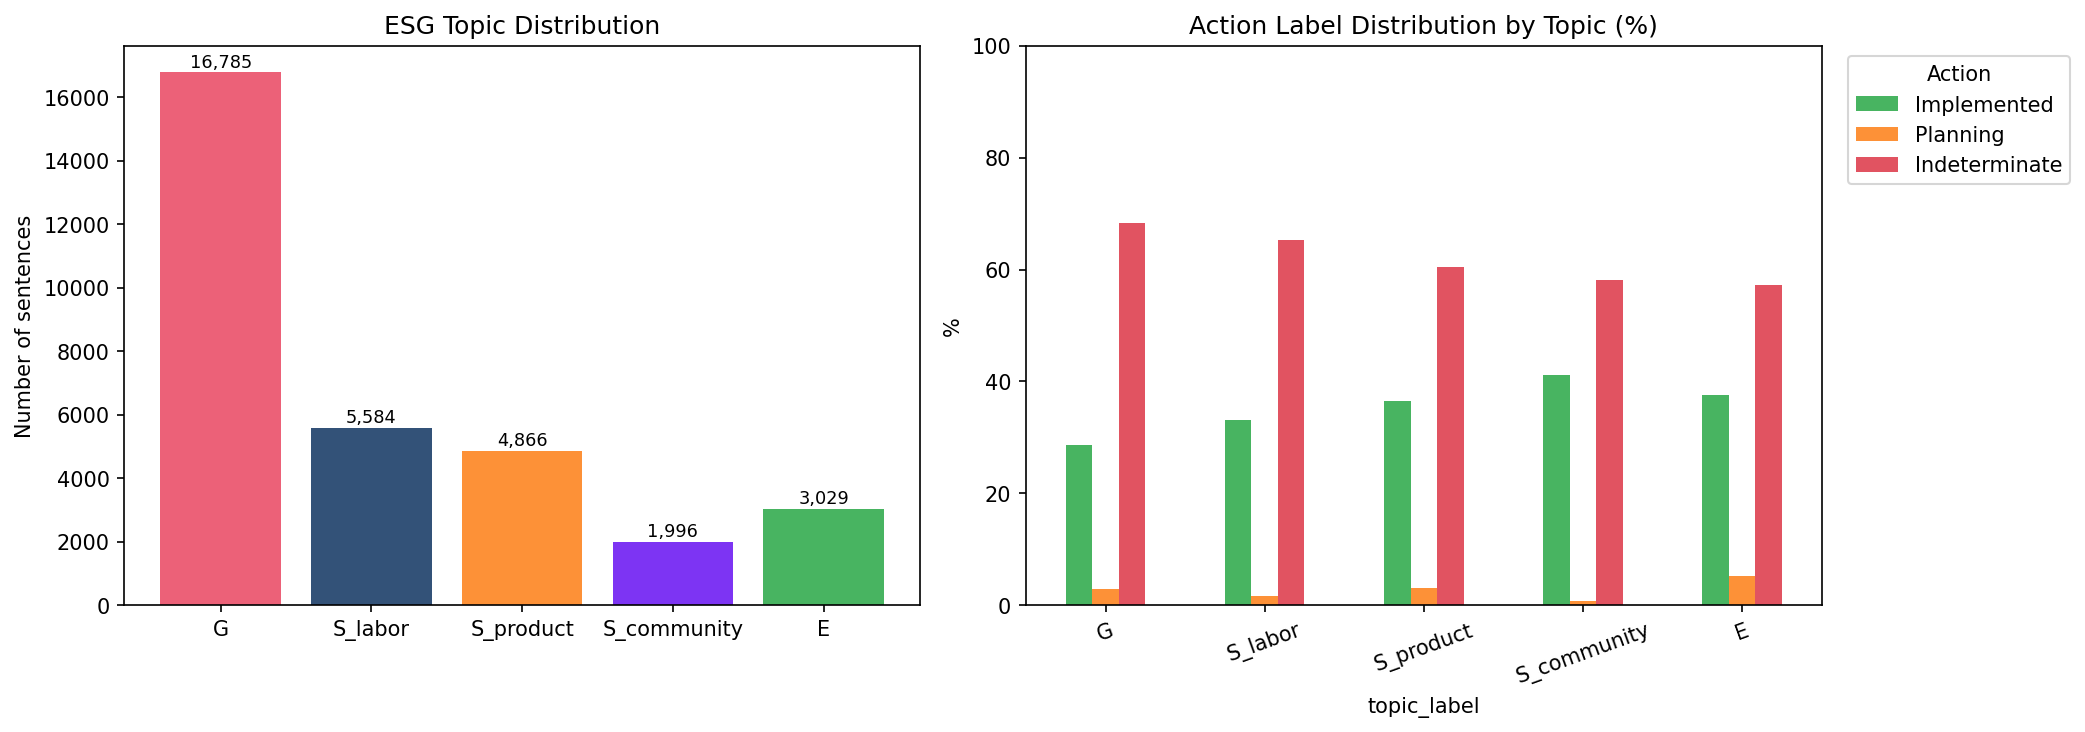
\includegraphics[width=0.95\textwidth]{figures/topic_distribution.png}
    \caption{Trái: Phân phối chủ đề ESG trong corpus (32.260 câu). Phải: Phân phối nhãn hành động theo từng chủ đề.}
    \label{fig:topic_distribution}
\end{figure}

Chủ đề G (Quản trị) chiếm tỉ trọng lớn nhất (52,0\%) và có EWRI cao nhất ($\approx 36$), phản ánh xu hướng các ngân hàng dành nhiều nội dung cho quản trị doanh nghiệp nhưng chủ yếu ở mức mơ hồ (68,4\% Indeterminate).

Chủ đề E (Môi trường) có tỉ lệ Planning cao nhất (5,2\%), cho thấy các ngân hàng có xu hướng đưa ra nhiều kế hoạch liên quan đến môi trường (cam kết giảm phát thải, lộ trình Net Zero) nhưng chưa có nhiều bằng chứng thực hiện.

Entropy chủ đề Shannon chuẩn hóa (Phương trình~\ref{eq:topic_entropy}) trên 50 quan sát ngân hàng-năm đạt trung bình $\bar{H} = 0{,}801$ ($\sigma = 0{,}094$), với biên độ $[0{,}566;\, 0{,}969]$. Giá trị trung bình gần 1 phản ánh các báo cáo nhìn chung đề cập tương đối đa dạng các chủ đề ESG. Tuy nhiên, một số quan sát có $H < 0{,}65$ cho thấy tình trạng tập trung quá mức vào G (chiếm 52,0\%) trong khi bỏ qua E và S\_product --- kết hợp với EWRI cao của G, đây là dấu hiệu của \textit{selective disclosure}: ngân hàng chủ động chọn chủ đề dễ trình bày mơ hồ để lấp đầy báo cáo~\cite{marquis2016scrutiny}.

Tóm lại chỉ số EWRI phản ánh phù hợp mức độ rủi ro ESG-washing trên 50 quan sát ngân hàng-năm. Kết quả cho thấy: Hệ thống phân biệt rõ ràng giữa 10 ngân hàng, với khoảng cách EWRI trung bình 10,95 điểm giữa nhóm tốt nhất (NH\_A, 31,77) và kém nhất (NH\_C, 42,72); Thành phần Indeterminate đóng góp đến 98,3\% tổng điểm EWRI, xác nhận đây là nguồn rủi ro washing chính trong báo cáo ESG ngân hàng Việt Nam.


% \subsection{Kiểm định độ tin cậy EWRI}
% \label{subsec:human_eval}

% Để kiểm định độ tin cậy của chỉ số WRS ở mức câu, nghiên cứu tiến hành thí nghiệm đánh giá chéo với người. 100 câu ESG được lấy mẫu ngẫu nhiên có phân tầng theo nhãn hành động (tỉ lệ tương đương phân phối thực tế: 60\% Indeterminate, 35\% Implemented, 5\% Planning), trình bày kèm bằng chứng liên kết (nếu có). Người thực hiện đánh giá chấm điểm rủi ro ESG-washing theo thang 1--5 (1 = rủi ro rất thấp / tuyên bố rõ ràng có kiểm chứng; 5 = rủi ro rất cao / tuyên bố mơ hồ không bằng chứng), không biết trước điểm WRS của hệ thống.

% \begin{table}[H]
% \centering
% \caption{Kết quả kiểm định tương quan WRS với đánh giá con người ($n = 100$).}
% \label{tab:human_eval}
% \begin{tabular}{lcc}
% \toprule
% \textbf{Độ đo} & \textbf{Hệ số} & \textbf{p-value} \\
% \midrule
% Pearson $r$     & 0,344 & $< 0{,}001$ \\
% Spearman $\rho$ & 0,441 & $< 0{,}001$ \\
% Kendall $\tau$  & 0,358 & $< 0{,}001$ \\
% \bottomrule
% \end{tabular}
% \end{table}

% Cả ba hệ số tương quan đều có ý nghĩa thống kê cao ($p < 0{,}001$), xác nhận WRS phản ánh đúng chiều xu hướng đánh giá rủi ro của con người. Mức Spearman $\rho = 0{,}441$ là kết quả xuất phát từ bản chất khác nhau của hai loại tín hiệu: WRS được tính hoàn toàn từ các tín hiệu hình thức --- nhãn hành động, sự hiện diện của bằng chứng (nhị phân), và phán định NLI --- trong khi con người đánh giá dựa trên hiểu biết ngữ nghĩa tổng thể, bao gồm cả ngữ cảnh rộng hơn ngoài câu đó. Nói cách khác, hai phía đang đo cùng một hiện tượng nhưng từ hai góc độ khác nhau, nên không thể kỳ vọng tương quan hoàn hảo. Mức tương quan này phản ánh đúng giới hạn nội tại của bài toán: WRS chỉ nhìn thấy thông tin hình thức trong một câu đơn lẻ (nhãn hành động, loại bằng chứng, phán định NLI), trong khi con người có thể huy động toàn bộ ngữ cảnh tài liệu và kiến thức nền để đưa ra phán đoán. Khoảng cách này là không thể lấp đầy bằng thiết kế công thức, mà chỉ có thể thu hẹp khi hệ thống được cung cấp thêm thông tin ngữ cảnh phong phú hơn.

% Phân tích sai lệch cho thấy không có trường hợp nào hệ thống đánh giá thấp khi người đánh giá cao (\textit{miss}: WRS $< 0{,}2$ và điểm $\geq 4$). Ngược lại, có 7 trường hợp hệ thống đánh giá cao hơn người (WRS $> 0{,}4$ nhưng điểm $\leq 2$), toàn bộ thuộc nhãn Indeterminate. Đây là các câu mà đánh giá viên nhận ra tính hợp lệ từ ngữ cảnh rộng hơn (ví dụ: đề cập đến chương trình quốc gia, phong cách hành chính đặc thù) mà hệ thống không nắm bắt được. Sự bất cân xứng này --- thiên về cảnh báo thừa hơn là bỏ sót --- thực tế phù hợp với mục tiêu ứng dụng: trong rà soát ESG-washing, bỏ sót rủi ro thực tế nghiêm trọng hơn cảnh báo thừa.

% Về xu hướng theo thời gian, phân tích EWRI trung bình qua các năm cho thấy bức tranh phức hợp: EWRI giảm rõ rệt từ 37,07 (2020) xuống 35,22 (2021), tương đương mức cải thiện 5,0\%, phản ánh bước tiến lớn trong chất lượng công bố ESG sau năm 2020 --- năm đầu tiên nhiều ngân hàng bắt đầu lồng ghép ESG vào báo cáo thường niên. Tuy nhiên, từ 2021 đến 2024, EWRI dao động quanh mức 35,2--36,9 mà không giảm thêm (2022: 35,95; 2023: 36,32; 2024: 36,88). Xu hướng này phản ánh rằng mức rủi ro ESG-washing đang đạt ``trạng thái ổn định'' --- các ngân hàng đã cải thiện bước đầu nhưng chưa có bước đột phá trong việc chuyển đổi từ công bố mơ hồ sang minh bạch có kiểm chứng.

\section{Phân tích định tính}
\label{sec:qualitative}

Để minh họa khả năng giải thích của hệ thống, phần này phân tích một số trường hợp cụ thể cho thấy pipeline hoạt động đúng ở cả hai cực rủi ro. Trường hợp rủi ro cao điển hình là câu \textit{``...chính sách và 02 chương trình mục tiêu quốc gia, xây dựng các sản phẩm tín dụng ưu đãi...''} (NH\_A, 2023, S\_product/Indeterminate, WRS = 0,550): không có bằng chứng đi kèm, thiếu KPI và mốc thời gian, ngôn ngữ mơ hồ tạo ấn tượng tích cực mà không cung cấp thông tin kiểm chứng. Ngược lại, câu \textit{``Tỷ trọng tín dụng xanh tại Ngân hàng [NH\_F] hiện đã lên tới hơn 10\%...''} (NH\_F, 2023, E/Implemented, WRS = 0,000) đạt rủi ro thấp nhờ ba yếu tố đồng thời: nhãn Implemented, bằng chứng KPI cụ thể (support = 1), và NLI xác nhận \textit{entailment}.

Bảng~\ref{tab:qual_examples} trình bày năm ví dụ đại diện từ các mức rủi ro và chủ đề khác nhau.

\begin{table}[H]
\centering
\caption{Năm ví dụ đại diện minh họa hoạt động pipeline. TBố: tuyên bố; BC: bằng chứng liên kết.}
\label{tab:qual_examples}
\footnotesize
\begin{tabular}{p{0.38\textwidth}p{0.15\textwidth}p{0.12\textwidth}p{0.07\textwidth}p{0.07\textwidth}p{0.07\textwidth}}
\toprule
\textbf{Nội dung (rút gọn)} & \textbf{Chủ đề / Hành động} & \textbf{Loại BC} & \textbf{NLI} & \textbf{support} & \textbf{WRS} \\
\midrule
\textit{TBố:} ``...chính sách và 02 chương trình mục tiêu quốc gia, xây dựng các sản phẩm tín dụng ưu đãi...'' \newline \textit{BC:} Không có
    & S\_product / Indeterminate & --- & --- & 0 & 0,550 \\
\midrule
\textit{TBố:} ``Chúng tôi sẽ tăng cường hợp tác với các đối tác quốc tế để thu hút nguồn vốn xanh, tích hợp các tiêu chuẩn ESG chặt chẽ hơn...'' \newline \textit{BC:} ``...nỗ lực này góp phần cải thiện môi trường sống...''
    & E / Planning & --- & neutral & 0 & 0,150 \\
\midrule
\textit{TBố:} ``96\% số lượng nhân viên có trình độ trên đại học đảm bảo nền tảng kiến thức chuyên môn...'' \newline \textit{BC:} \textit{(câu tương tự trong ngữ cảnh khác)}
    & S\_labor / Implemented & KPI & entail. & 1 & 0,000 \\
\midrule
\textit{TBố:} ``[NH\_F] đã hoàn tất 03 trụ cột của Hiệp ước vốn Basel II từ năm 2020 và tiếp tục triển khai theo phương pháp nâng cao...'' \newline \textit{BC:} ``[NH\_F] cũng đã hoàn tất 03 trụ cột Basel II từ năm 2020, đáp ứng tuân thủ toàn diện...''
    & G / Implemented & Std, Time & entail. & 1 & 0,000 \\
\midrule
\textit{TBố:} ``Tỷ trọng tín dụng xanh tại Ngân hàng [NH\_F] hiện đã lên tới hơn 10\% trên tổng danh mục cho vay...'' \newline \textit{BC:} \textit{(câu tương tự xác nhận)}
    & E / Implemented & KPI & entail. & 1 & 0,000 \\
\bottomrule
\end{tabular}
\end{table}

Các ví dụ trên cho thấy pipeline hoạt động đúng qua ba khía cạnh: (1) \textit{Phân loại hành động}: hệ thống phân biệt chính xác giữa ngôn ngữ mơ hồ (``chính sách'', ``chương trình mục tiêu'' $\to$ Indeterminate), ngôn ngữ kế hoạch (``sẽ tăng cường'' $\to$ Planning), và ngôn ngữ đã thực hiện (``đã hoàn tất'', ``đã lên tới'' $\to$ Implemented). (2) \textit{Liên kết bằng chứng}: hệ thống tìm được bằng chứng tương đồng ngữ nghĩa từ ngữ cảnh tài liệu; câu Implemented có bằng chứng hỗ trợ (support = 1), trong khi câu Indeterminate/Planning thiếu bằng chứng (support = 0). (3) \textit{NLI verification}: mô hình NLI xác nhận \textit{entailment} cho các cặp tuyên bố-bằng chứng thực sự hỗ trợ nhau (ví dụ: ``đã hoàn tất 03 trụ cột Basel II'' và bằng chứng xác nhận cùng nội dung), trong khi đánh giá \textit{neutral} cho các cặp có liên quan chủ đề nhưng không trực tiếp xác nhận.

\section{Thảo luận}
\label{sec:discussion}

Lagasio~\cite{lagasio2024esg} xây dựng ESGSI dựa trên TF-IDF và LDA để đo mật độ từ vựng tích cực trong báo cáo ESG. Cách tiếp cận này, dù đơn giản nhưng lại có điểm yếu là nó đếm \textit{từ ngữ}, không đánh giá logic. Một đoạn văn dài dòng, sáo rỗng, chứa nhiều thuật ngữ ESG nhưng không có cam kết cụ thể nào vẫn được ghi nhận điểm cao. Phương pháp đề xuất trong nghiên cứu này đòi hỏi \textit{tính kiểm chứng ngữ nghĩa}: bằng chứng chỉ được tính khi mô hình NLI phán định \textit{entailment} --- nghĩa là văn bản bằng chứng phải \textit{suy ra được} tuyên bố, không chỉ liên quan về chủ đề. Điều này giúp hệ thống chống lại được kỹ thuật ``thổi phồng'' ngôn ngữ mà các phương pháp thống kê không phát hiện được.

Florstedt và Fahlbusch~\cite{florstedt2025detecting} đã tiến hành phân tích mức câu và liên kết bằng chứng nội tại. Điểm bổ sung quan trọng của nghiên cứu này so với công trình đó là chiều thông tin \textit{mức độ hành động} (Implemented / Planning / Indeterminate) --- một trục phân tích mà Florstedt et al.\ không xét đến. Kết quả thực nghiệm cho thấy trục này giải thích tới 89,30\% phương sai của điểm rủi ro ở mức câu (ANOVA $\eta^2 = 0{,}893$), chứng tỏ rằng câu hỏi ``hành động này đã xảy ra chưa?'' quan trọng hơn câu hỏi ``có bằng chứng kèm theo không?'' trong việc phân biệt cam kết thực chất với ngôn ngữ hứa hẹn.

Nghiên cứu này đã đưa ra và kiểm chứng thực nghiệm một luận điểm có ý nghĩa: \textit{ở các thị trường mới nổi thiếu vắng dữ liệu xếp hạng ESG từ bên thứ ba độc lập, khả năng kiểm chứng nội tại của văn bản là một đại lượng thay thế đáng tin cậy để đo lường rủi ro ESG-washing.}

Một đóng góp lý luận thứ hai liên quan đến hướng ứng dụng Neuro-Symbolic AI. Nghiên cứu cho thấy các mô hình ngôn ngữ lớn không nhất thiết phải vận hành như ``hộp đen''. Bằng cách tích hợp tri thức chuyên gia dưới dạng ràng buộc ký hiệu trực tiếp vào hàm mất mát --- cụ thể là các quy tắc loại trừ lẫn nhau từ GRI và các khung phân loại ESG của Bloom và Hyland --- mô hình được định hướng học các ranh giới nhãn phù hợp với chuẩn mực ngành, thay vì chỉ tối ưu hóa thuần thống kê. Kết quả là Neuro-Symbolic đạt Macro F1 = 0,832 (chủ đề) và 0,821 (hành động), vượt trội Baseline trên toàn bộ nhãn, trong đó cải thiện rõ nhất ở các nhãn thiểu số có ranh giới mờ (Planning, S\_community). Điều này gợi ý rằng đối với các bài toán phân loại văn bản chuyên ngành có tri thức phong phú, hướng neuro-symbolic đáng được nghiên cứu tiếp như một lựa chọn có khả năng giải thích cao hơn so với tinh chỉnh mô hình đơn thuần.